\documentclass[a4paper]{article}

%text
%\usepackage[utf8]{inputenc}
%\usepackage[numbers,super]{natbib}
%\usepackage{lipsum}
%\usepackage{amssymb,amsmath}
%\usepackage{gensymb}
%\usepackage{listings}
%\usepackage{amsfonts}
%\usepackage{todonotes}
%\usepackage{listings}
%\usepackage{scrextend}
%graphics
%\usepackage{graphicx, xcolor}
%\usepackage{rotating}
%\usepackage{subfig}
%\usepackage{float}
\usepackage[top=.8in, bottom=1.0in, left=1.in, right=.7in]{geometry}



\usepackage[utf8x]{inputenc}
\usepackage[swedish,english]{babel}
\usepackage[colorlinks=true,linkcolor=black]{hyperref}
\usepackage{listings}
\usepackage{color} %red, green, blue, yellow, cyan, magenta, black, white
\definecolor{mygreen}{RGB}{28,172,0} % color values Red, Green, Blue
\definecolor{mylilas}{RGB}{170,55,241}

\usepackage{listings}
\usepackage{hyperref}
\usepackage{bookmark}

\usepackage{siunitx}  % Provides the \SI{}{} command for typesetting SI units
\usepackage{graphicx} % Required for the inclusion of images
\usepackage{amsmath}
\usepackage{gensymb}
\usepackage{amsfonts}
\usepackage{amssymb}
\usepackage{subcaption}
\usepackage{tabularx}
\usepackage{dcolumn}
\usepackage{booktabs}
\usepackage{hyperref}
\usepackage{graphicx}
\usepackage[swedish]{babel}
\graphicspath{ {images/} }
\graphicspath{ {/Users/johanbjork/Documents/F0008T/hemuppgift} }
\usepackage{float}
\usepackage{commath}


  %FÖR MATLABKOD!
 
\usepackage[framed,numbered,autolinebreaks,useliterate]{mcode}

% links
\usepackage{color}
\usepackage[linktocpage=true, colorlinks=true, allcolors=blue]{hyperref}
\usepackage[all]{hypcap}
\usepackage[hypcap]{caption}

%layout
\usepackage{multicol}
\usepackage{fancyhdr,lastpage}
\setcounter{tocdepth}{2}

%header layout
\usepackage{suffix}
\newcommand{\project}{\emph {SailorAid}}

\newcommand\chapterauthor[1]{\authortoc{#1}\printchapterauthor{#1}}
\WithSuffix\newcommand\chapterauthor*[1]{\printchapterauthor{#1}}

\makeatletter
\newcommand{\printchapterauthor}[1]{%
  {\parindent0pt\vspace*{-10pt}%
  \linespread{1.1}\large\scshape#1%
  \par\nobreak\vspace*{10pt}}
  \@afterheading%
}
\newcommand{\authortoc}[1]{%
  \addtocontents{toc}{\vskip-1pt}%
  \addtocontents{toc}{%
    \protect\contentsline{chapter}%
    {\hskip0em\mdseries\scshape\protect\scriptsize#1}{}{}}
  \addtocontents{toc}{\vskip5pt}%
}
\makeatother



%header style
\pagestyle{fancy}
\lhead{Project \project}
\chead{}


\rhead{\today}
\lfoot{}
\cfoot{\thepage~of~\pageref{LastPage}}
\rfoot{}
\renewcommand{\headrulewidth}{0.4pt}
\renewcommand{\footrulewidth}{0.4pt}

\begin{document}

\begin{titlepage}
\newcommand{\HRule}{\rule{\linewidth}{0.5mm}}
\center % Centre everything on the page

%------------------------------------------------
%	Headings
%------------------------------------------------

\textsc{\LARGE Luleå University of Technology}\\[1.5cm] % Main heading such as the name of your university/college

\textsc{\Large Dept. of Computer Science, Electrical and Space Engineering}\\[0.5cm] % Major heading such as course name

\textsc{\large D7039E -- Project in Industrial Computer Systems}\\[0.5cm] % Minor heading such as course title

%------------------------------------------------
%	Title
%------------------------------------------------

\HRule\\[0.8cm]

{\huge\bfseries Project \project}\\[0.4cm] % Title of your document

\HRule\\[1.5cm]

%------------------------------------------------
%	Author(s)
%------------------------------------------------
\begin{minipage}{0.4\textwidth}
	\begin{flushleft}
		\large
		\textit{Authors}\\
		Axelsson Oskar, \\ 
		Brolin, Daniel, \\ 
		Eriksson, Kenny \\ 
		Grape, Elias \\ 
		Lundberg, Josef, \\ 
		Sjölund, Johannes \\
		Theolin, Henrik
	\end{flushleft}
\end{minipage}
~
\begin{minipage}{0.4\textwidth}
	\begin{flushright}
		\large
		\textit{Supervisor}\\
		van Deventer, Jan
	\end{flushright}
\end{minipage}

% If you don't want a supervisor, uncomment the two lines below and comment the code above
%{\large\textit{Author}}\\
%John \textsc{Smith} % Your name

%------------------------------------------------
%	Date
%------------------------------------------------

\vfill\vfill\vfill % Position the date 3/4 down the remaining page

{\large\today} % Date, change the \today to a set date if you want to be precise

%------------------------------------------------
%	Logo
%------------------------------------------------

\vfill\vfill
\includegraphics[width=0.2\textwidth]{Figures/ltu.jpg}\\[1cm] % Include a department/university logo - this will require the graphicx package
 
%----------------------------------------------------------------------------------------

\vfill % Push the date up 1/4 of the remaining page


\end{titlepage}

\clearpage
\begin{abstract}
Some abstract description of the project... 
\lipsum[4-5]
<<<<<<< HEAD
ffffsds
=======
>>>>>>> 45c398972e2e2e028b4e97cae9c2f2561abfb42b

\end{abstract}

\clearpage
\setlength{\columnseprule}{0.2pt}

\tableofcontents

\vspace{0.5em}

\clearpage

\setcounter{page}{2}
\section{Introduction}
\chapterauthor{who??? (no one)}
% \lipsum[7-8]
% - Is this too general? Feels too much like a very long abstract

% - "While slipping across the waves... " This is just a weird sentence, but I can't put my finger on it
%   Put paragraph-break before this sentence?
% - "compact, portable and simple" OR "compact, portable, simple"
The art of sailing has been around for millennia. For much of human history it has been an absolutely vital part of civilization, providing efficient means of transporting goods all around the world. Today sailing has become a leisure activity enjoyed by millions of people around the world. Modern sailboats come in a large span of sizes, from large ships with crews of dozens down to small single-man dinghies. While slipping across the waves out at sea with only the wind to drive you is a calming experience, it is not a simple thing to do. When you are alone on the water, you have to be in control of the tension of the sail, the attitude of the boat, the forces on the centerboard and more while deciding how to respond to all of these. The goal of Project \emph{SailorAid} is to offload the decision-making from the sailor onto a compact, portable and simple system that will analyze these parameters and provide clear directions to the \gls{skipper}. 

% - Put this section after Physics of Sailing to give context to the goals?
% - Have goals in it's own subsection or incorperate into introduction? Or move it into Product Application?
%   And what should Product Application contain? What the product does or how it is put on the boat?
% - "The primary functional..." is too short and mechanical. Try to write something more organic later
\subsection{Goals}
The primary functional goals are the following:
\begin{itemize}[noitemsep] % For consistency the item layout is reverted to standard.
	\item Boat attitude
	\begin{itemize}[noitemsep]
		\item Implementing an appropriate \gls{imu}:
		\begin{itemize}[noitemsep]
			\item Accelerometer
			\item Gyroscope
			\item Magnetometer
		\end{itemize}
		\item Fusing the sensor output to get an accurate estimate of boat attitude
	\end{itemize}
	\item Position tracking and velocity
	\begin{itemize}[noitemsep]
		\item Implementing a \gls{gps} system
		\item Fusing the \gls{gps} output with the accelerometer output for more accurate positioning and velocity
	\end{itemize}
	\item Design a force measurement circuit for the centerboard
	\begin{itemize}[noitemsep]
%		Rephrase item 1, "off the centerboard" might be ambiguous. Intent: "off" as in "not mounted on" but that feels clumsy. But "not mounted on" might work if it has been made clear earlier why we can't put it on the centerboard.
		\item Design an appropriate sensor mount off the centerboard
		\item Implement an appropriate sensor
		\item Implement a centerboard-depth sensor
	\end{itemize}
	\item  Feedback to the user of the system
	\begin{itemize}[noitemsep]
		\item Give the user information from the sensors
		\item Display instructions to help improve the sailing experience depeding on the system state
		\item Implement different ways for the user to retrieve information
	\end{itemize}
\end{itemize}



\section{The Physics of Sailing}
\label{sec:physics}
\chapterauthor{Henrik, Theolin (Oskar, Axelsson)}
\subsection{Point of sail}
A sailboat can achieve velocity by catching the wind in the sail at different angles. This is called point of sail and the velocity is dependent on the dinghies displacement from the true wind direction, the wind experienced for a stationary object, where the velocity is a resultant of the force vector created by the wind depending on the alignment of the sail and the direction from the wind direction. There are five different states of point of sail that are divided into degrees away from the true wind origin. These are
\begin{labeling}{alligator}
\item [Luffing] (no propulsive force) angle between 0-30\degree
\item [Close-hauled] (lift) angle between 30-50\degree
\item [Beam reach] (lift) angle 90\degree
\item [Broad reach] (lift–drag) angle aound 135\degree
\item [Running] (drag) angle around 180\degree
\end{labeling}
and are represented in Fig. \ref{points-sail}. A sailor wants to prevent the sail from luffing, luffing is when the sail starts to flap in the wind and no propulsive force is achieved. When the dinghy is in the close-hauled and beam reach state the sail produces lift force that is produced from the average pressure differences on the windward and leeward side of the sail where the pressure is higher on the windward surface thus acting like a wing propelling the dinghy. When the dinghy is in the broad reach state both lift and also drag propels the dinghy. Drag acts like a parachute that that catches the wind and propels the dinghy. The sideway force induced on the boat also introduces drift perpendicular to the relative bearing. This is counteracted by lowering a centerboard which also counteracts the dinghy from heeling.
\begin{figure}[H]
\centering
\includegraphics[width=0.6\textwidth]{Figures/Points_of_sail.jpg}
\caption{Points of sail}
\label{points-sail}
\end{figure}
\begin{figure}[H]
\centering
\includegraphics[width=0.6\textwidth]{Figures/max_lift.jpg}
\caption{Sail angles of attack}
\label{max_liftl}
\end{figure}
\subsection{Velocity}
The main goal in sailing is to maximize the efficiency at which the forces on the sail translates into the velocity of the dinghy. A layman might expect that the fastest velocity is achieved when the dinghy is parallel to the true wind, however, this is not true. The apparent wind which is the wind experienced from the dingy perspective is what propels the dingy. When sailing parallel to the wind the dinghies speed can never exceed the speed of the wind\cite{sail-force}. By sailing upwind close-hauled the apparent wind is increased as the dingy accelerates until the drag from the water exceeds the forward force created by the wind. To further increase the velocity of the dingy should not be heeling excessively. This is to prevent the centerboard from acting as a rudder and changing the bearing, introducing more drag from the stern rudder when compensating for the bearing changes. As mentioned earlier the centerboard helps to counteract heeling but also the sailor can prevent this by hiking, leaning outside of the hull to alter the center of mass for the dinghy. Lastly when all other measures were taken the sailor must perform reefing and reducing the area of the sail and lowering the center of effort from the sails.


\section{Product Application}
\label{sec:application}
\lipsum[9]

\subsection{Navigation and Tracking}
\chapterauthor{Sjölund, Johannes (Theolin, Henrik)}
\lipsum[10]

\subsection{Speed optimization}
\chapterauthor{Sjölund, Johannes (Theolin, Henrik)}
\lipsum[11]


\section{Hardware Design}\label{sec:hwdesign}
\chapterauthor{Brolin, Daniel (one, no)}
This chapter will summarize most of the process of creating the \gls{pcb} used to mount all the sensors and sending the data to the phone application. This circuit board will be the link between the physical forces and manipulated data sent to the handheld device. More on how this data is manipulated and how the circuit board is programmed in \autoref{sec:sw}. 

The circuit board must minimally fulfill the following set of basic requirements to function properly:
\begin{itemize}[noitemsep]
\item Circuit must fit within the casing, with dimensions extracted directly from the cad software\cite{cad}, see \autoref{fig:casdim}.
\item Circuit must be easy to test for both hardware and software errors. Even complete system needs this, since many of the sensors are very small and difficult to solder.
\item All sensors must fit on the \gls{pcb}, both physically and also electronically on the ports of the \gls{mcu}.
\item Must be protected against all common problems, such as overcharge, undercharge, capacitive effects, and more.
\item All components needs to be actively manufactured to ensure unit can keep being produced for several years in the future.
\end{itemize}

\subsection{Method}
% Methodology
The main circuit board is built using the open source electronic design software KiCad\cite{kicad}. It is completely free to use and the source code is open for any modifications.
Designing circuit boards differs slightly between what software you are using. KiCad\cite{kicad} uses a four step process as follows:
\begin{enumerate}[noitemsep]
\item Draw schematic:
	\begin{enumerate}[noitemsep]
	\item Place and connect all components.
	\item (Optional:) All non-standard components must be custom designed, this is referred to as ``library''. Most sensors requires custom built libraries.
	\item Annotate schematic and run \gls{erc} to identify simple electronic violations.
	\end{enumerate}
\item Create net-list:
	\begin{enumerate}[noitemsep]
	\item (Optional:) All components with non-standard (or simply not standard enough) footprints must be custom designed, these include all sensors and the \gls{bt} module.
	\item Associate all components with whatever physical footprint are to be used.
	\item Generate net-list.
	\end{enumerate}
\item Design \gls{pcb} layout:
	\begin{enumerate}[noitemsep]
	\item Import net-list to \gls{pcb} editor.
	\item Set global and net-specific design rules.
	\item Place and connect all components.
	\item Run \gls{drc} to identify all specified design rule violations.
	\end{enumerate}
\item Generate manufacturing (gerber/drill) files.
\end{enumerate}
% Borrowed shit
The initial required circuitry, see \autoref{fig:schr3a}, was copied from earlier works with the \gls{st} \gls{arm} \gls{mcu}'s but modified to meet our needs. The power section, also found in \autoref{fig:schr3a}, is designed to only allow for exactly $+5V$. This design is credited to, and derived from \emph{Maxim Integrated}, Application note 760\cite{overprotection}.

% Original custom shit
Non-standard library entries include following components:\\
\begin{minipage}{\linewidth}
\begin{table}[H]
\centering
	\begin{tabular}{ l | l | l | l }
 	Name		& Type 								& Library 				& Used in         \\
 			&									&					& last rev.\footnote{revision}\\\hline
  	A2235-H  	& \gls{gps} 								& a2235-h.lib 			& \textbf{YES}\\
  	FT232RL 	& USBtoSerial converter 						& ftdi.lib\cite{ftdi}			& \textbf{YES}\\
  	HTS221 	& Humidity sensor 							& Custom\_sensors.lib 		& \textbf{YES}\\
  	LM1117ADJ 	& Voltage Regulator						& PowerSupply.lib\cite{lm1117} 	& \textbf{YES}\\
  	LPS22HB 	& Pressure sensor  							& Custom\_sensors.lib 		& \textbf{YES}\\
  	LSM303AGR	& Acc.\footnote{Accelerometer}/Mag.\footnote{Magnetometer} \gls{imu} & Custom\_sensors.lib & \textbf{YES}\\
  	LSM303Cx 	& Acc./Mag. \gls{imu} 						& Custom\_sensors.lib		& \textbf{NO} \\
  	LSM6DSL 	& Acc./Gyro.\footnote{Gyroscope} \gls{imu} 			& Custom\_sensors.lib 		& \textbf{YES}\\
  	LSM9DS1 	& Acc./Gyro./Mag. 							& Custom\_sensors.lib 		& \textbf{NO} \\
  	MCDTS2-4N 	& Tactile switch button 						& Custom\_Switches.lib 		& \textbf{YES}\\
\end{tabular}
\caption{Non-standard library entries custom or third-party designed}
\label{table:nstdlibs}
\end{table}
\end{minipage}

%\subsection{Revisions}\label{sec:hw:rev}
In total three revisions of the \gls{pcb} was designed. The first revision was designed well before any components arrived and was meant exclusively as a prototype, while both the second and third revisions were supposed to have full functionality. All revisions following the first were initially supposed to be designed as consecutive debugged states, but complete redesigns of component placings and tracing was eventually necessary.

\subsubsection{First revision}
First revision included the main functionality and test points on basically every pin in the system. It did not follow any space- or requirements and was riddled with small problems. The USBtoSerial converter was broken, the \gls{i2c} line was short circuited somewhere, the custom footprint for the \gls{gps} was mirrored, the \gls{bt} worked, but poorly due to inferences from other circuitry and so on and so fourth. Most of this was probably because we had to design the \gls{pcb} and draw all custom made footprints before actually receiving the components. This revision was also meant as a prototype, and not enough time was put to make sure all isolation's and trace widths had well thought out values. A high-speed switching logic had been designed for the wakeup-signal to the \gls{gps}, but this was not used. The schematic of revision one has not been included in this report, as there is little to learn from it; the \gls{pcb} can however be seen as \autoref{fig:pcbr1}.
\begin{figure}[tbh]
	\centering
    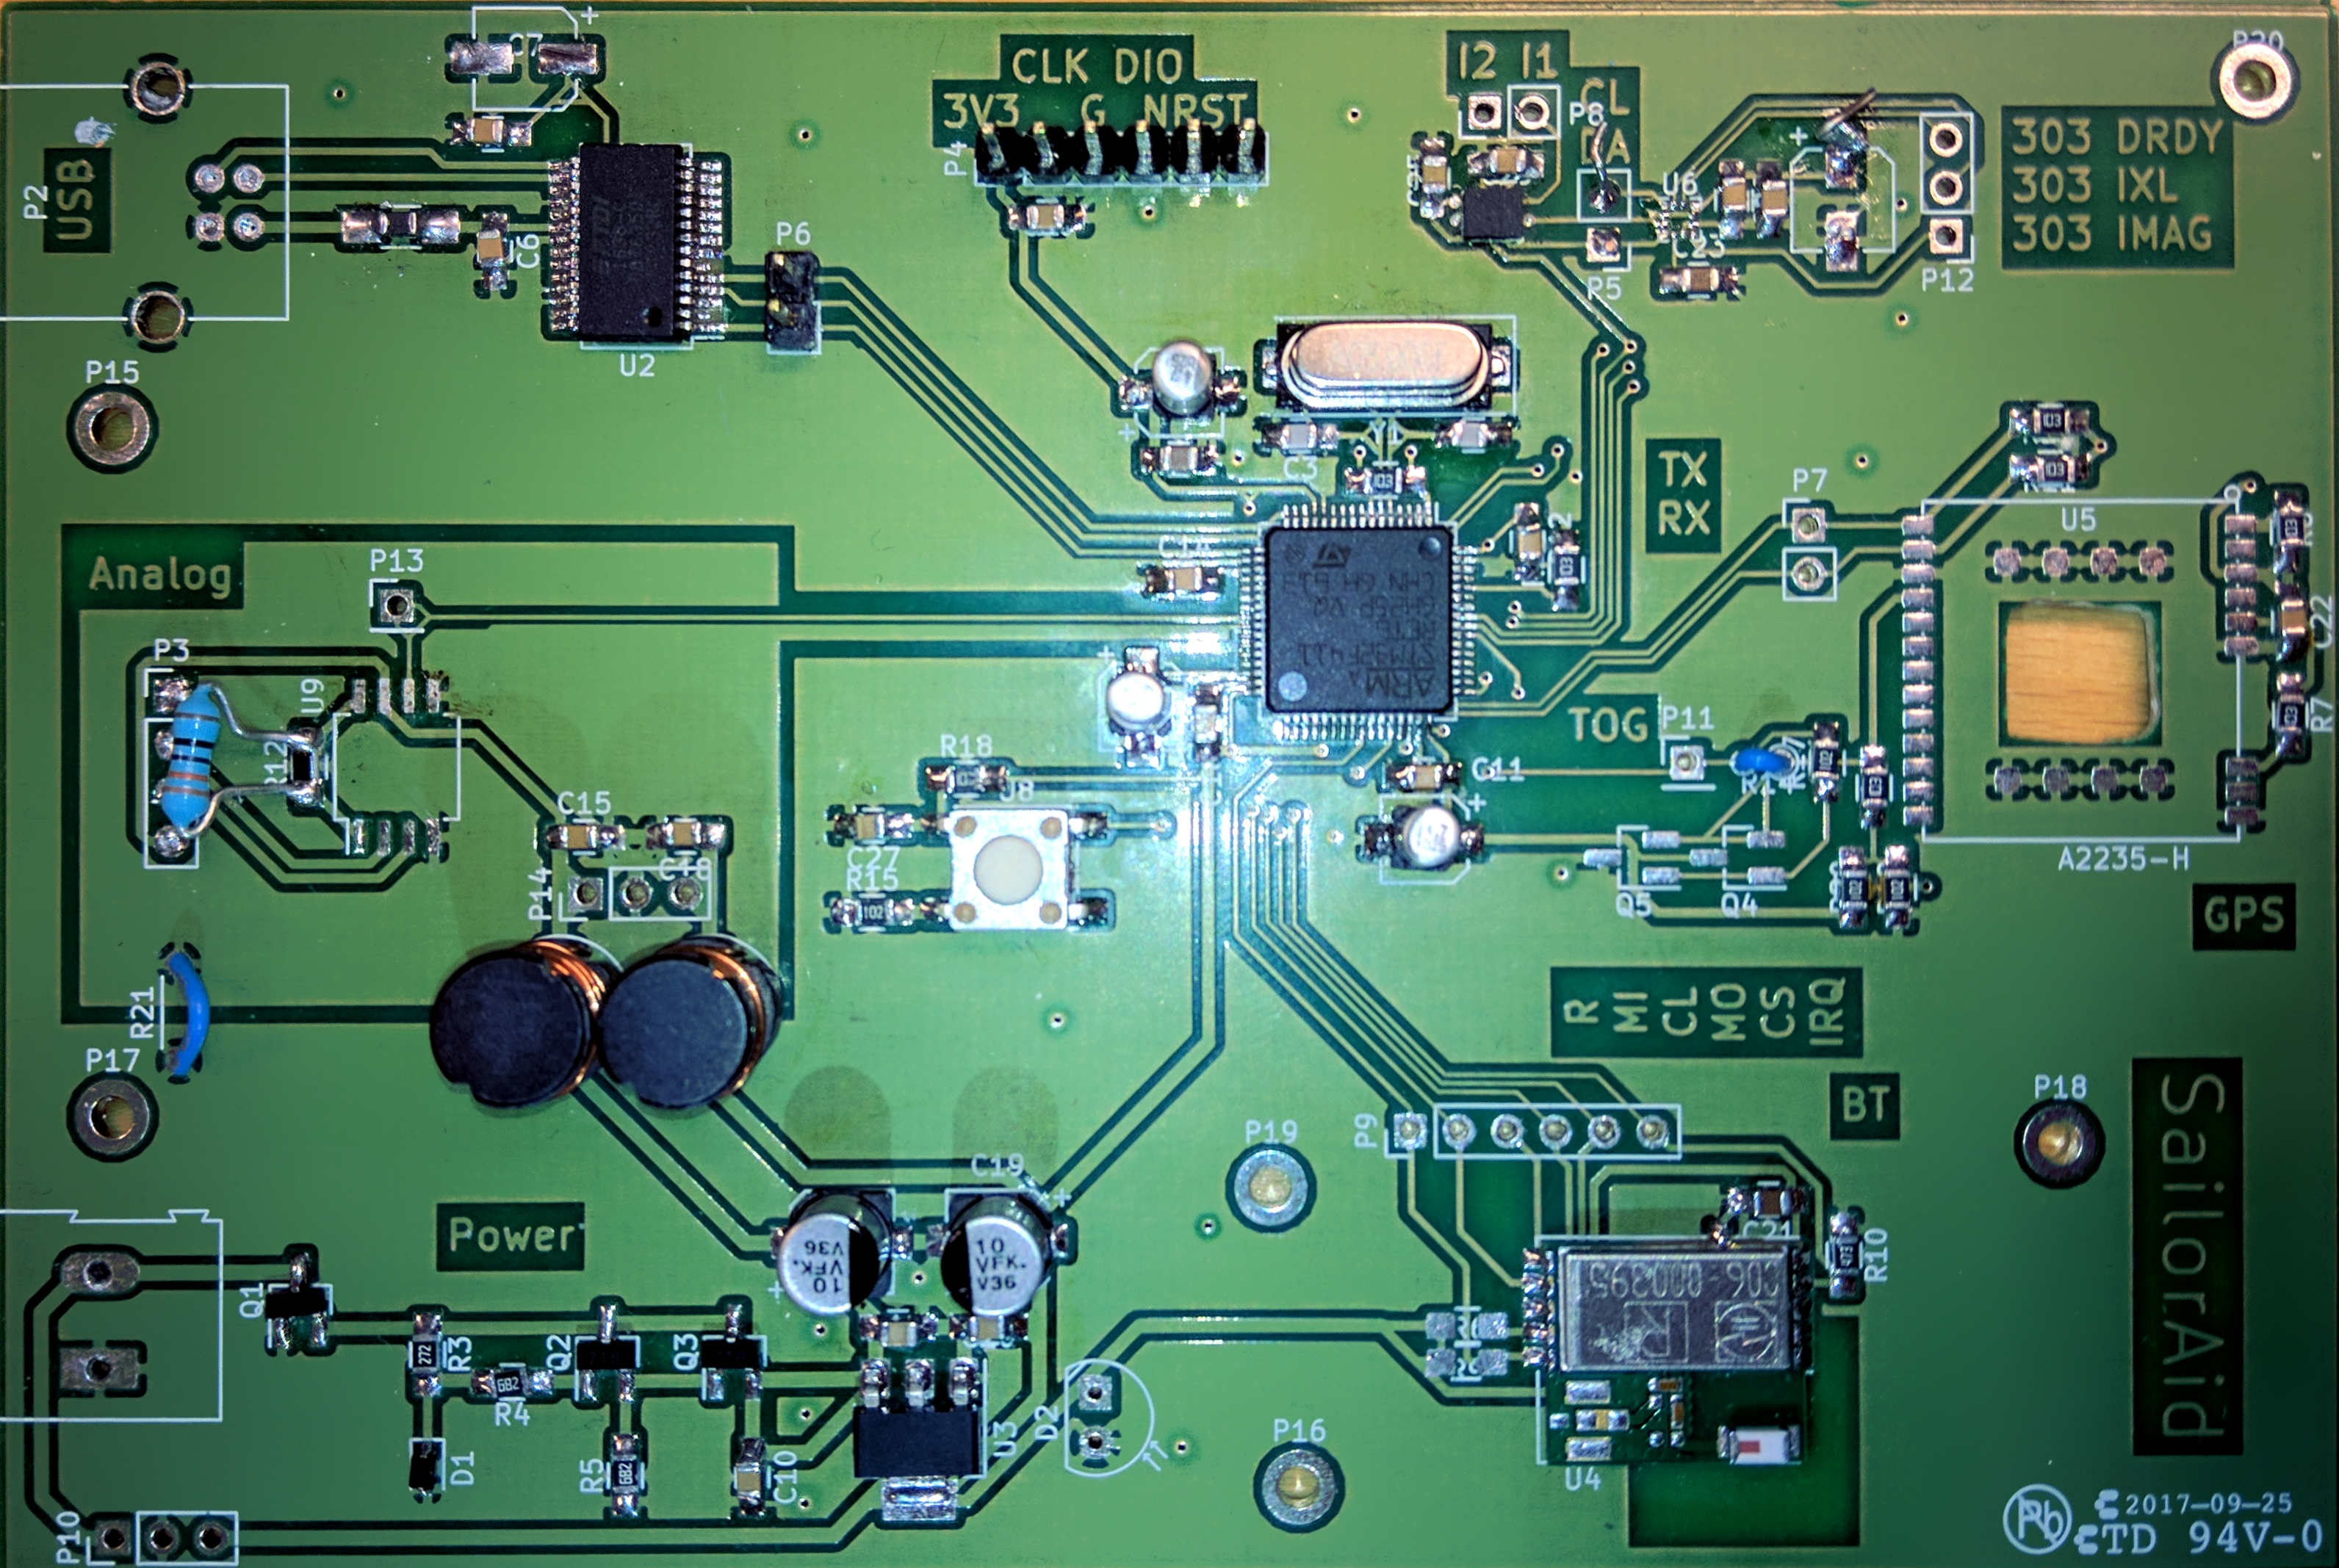
\includegraphics[width=\linewidth]{Figures/pcb_rev1.jpg}
	\caption{First (1) revision circuit board}
	\label{fig:pcbr1}
\end{figure}

\subsubsection{Second revision}
The second revision fixed all known problems, followed the space requirements and added a lot of customization. The option to toggle power source and what \gls{imu}s were currently powered were added. This way the effect from individual modules could be measured. Also since it was still unclear if a combined chip for all \gls{imu}s would be added or not, space for all of them and an evaluation module was added. However, some wires was lost in the transition from revision one to two, as all net-labels in the schematic was redrawn; also the micro-\gls{usb} housing was to small for continuous use and was ripped of by our, way to strong, programmers; all of this was hot fixed and eventually the circuit board worked as expected. As with revision one, the schematic of revision two has not been included in this report, as there is little to learn from it; the \gls{pcb} can however be seen as \autoref{fig:pcbr2}.
\begin{figure}[tbh]
	\centering
	\includegraphics[width=\linewidth]{Figures/pcb_rev2.jpg}
	\caption{Second (2) revision circuit board}
	\label{fig:pcbr2}
\end{figure}

\subsubsection{Third revision}
With almost all problems solved in the second revision, what remained was some hotfix for an unexpected wiring error in the \gls{gps}; interference between \gls{i2c} clock and data line; minimizing much to large decoupling ground loops; unwanted antennas; ground islands of missing copper and a KiCad problem where disconnected \gls{via}s lose their net property. The option to pull power from either \gls{usb} or batteries remained in the last revision, as this makes programming and testing much easier. A four pin connector to measure the battery level through \gls{i2c} was added, and since the power level of this depends slightly on the power left in the batteries logic level converters was designed to allow for a variable voltage level\cite{llc}, the electronic circuitry can be see in \autoref{fig:schr3b}.
For the third revision all decisions have been made and the schematic can be seen as \autoref{fig:schr3a}, \ref{fig:schr3b} and \ref{fig:schr3c}.

Following communicative devices will used and act as ``mudule areas'', i.e. these units will be the central units of the \gls{pcb} layout. This was introduced in the second
\begin{itemize}[noitemsep]
\item{\makebox[3cm][l]{STM32F411RET} - Microcontoller unit}
\item{\makebox[3cm][l]{FT232RL} - \gls{usb}toSerial converter (USART)}
\item{\makebox[3cm][l]{A2235-H} - \gls{gps} unit (UART)}
\item{\makebox[3cm][l]{SPBTLE-RF} - \gls{bt} connection unit (SPI)}
\item Sensors ($I^2C$):
	\begin{itemize}[noitemsep]
	\item{\makebox[3cm][l]{LSM303AGR} - Accelereometer \& Magnetometer}
	\item{\makebox[3cm][l]{LSM6DSL} - Accelerometer \& Gyroscope}
	\item{\makebox[3cm][l]{HTS221} - Humidity}
	\item{\makebox[3cm][l]{LPS22HB} - Pressure}
	\end{itemize}
\item Sensors, connectors only ($I^2C$):
	\begin{itemize}[noitemsep]
	\item Battery level
	\item VL530x \qquad- Time of flight
	\end{itemize}
\item INA128 \qquad- Analog load cell amplifiers (ADC)
\item MCDTS2-4N \qquad- Tactile push buttons (Pull-up/Pull-down)
\end{itemize}
The layout of the components are such that all \gls{i2c} communicative devices are moved to one spot ensuring the shortest possible \gls{i2c} data line, these are placed to the top right of the \gls{pcb}. The power is placed in the bottom left, since this is as far as possible from everything else. \gls{usb} is placed next to the power, as power can be opted to be drawn from \gls{usb} rather than battery. Analog plane with the load cells are put right next to the power to ensure the star-ground\footnote{A common node ground connecting all grounds together to ensure the same set working level} to be as close as possible to the power-source allowing for as little noise as possible. \gls{bt} communication devices are rather fragile, it is therefore placed as far as possible from everything in the top left corner of the \gls{pcb}. This \gls{bt} module (SPBTLE-RF) requires \gls{spi} communication and in total $6$ isolated traces are to be drawn between the \gls{mcu} and the \gls{bt} unit. To minimize crossover the \gls{gps} is placed in the top-mid of the \gls{pcb}. Lastly the buttons whose placing is of low importance are placed in the middle-left, between the power source and the \gls{bt} unit. 
Ground \gls{via}s was added around communication traces to prevent unwanted interference, ground \gls{via}s were also added to prevent antennas\footnote{Antennas appear by letting isolated thin grounds be connected on only one end, a \gls{via} can therefore be added to the other end to prevent this from happening.}.
The third, and last, revision of the \gls{pcb} can be seen in \autoref{fig:pcbr3}, a simple explanation of the layout can be seen in \autoref{fig:pcbr3simple}.
\begin{figure}[tb]
	\centering
    \includegraphics[width=\linewidth]{Figures/pcb_rev3.jpg}
	\caption{third (3) revision circuit board}
	\label{fig:pcbr3}
\end{figure}
\begin{figure}[tb]
	\centering
    \includegraphics[width=.75\linewidth]{Figures/pcb_rev3_simple.png}
	\caption{Simple model of third (3) revision circuit board areas}
	\label{fig:pcbr3simple}
\end{figure}

\subsection{Component choices}\label{sec:hw:tip1}
\chapterauthor*{Eriksson, Kenny (Brolin, Daniel)}
In order to choose what components would be used for the system, the first consideration was the central controller of the system. Because the system was designed to work in conjunction with an app on a smartphone it was agreed that there is no need for heavy computation on the on-board module. This meant that a \gls{mcu} would be sufficient. Because several of the project members had previous experience with the \gls{st} brand \emph{STM32F411RE} and it has a significant number of GPIO ports, useful peripherals (\gls{i2c}, \gls{spi}, timers, etc) and a high clock speed of up to $100~\textrm{MHz}$ it was chosen as the core of the on-board module. 

The \emph{STM32F411RE} utilizes the \gls{swd} protocol for programming and debugging, the programmer in this case being the programming section of a \emph{NUCLEO-F411RE} development board configured as a programmer. The \gls{swd} header also provides a \gls{uart} channel to communicate with the \gls{mcu}. However, in the interest of convenience for the developers a \emph{FT232RL} chip was added. The \emph{FT232RL} is a \emph{\gls{usb}-to-\gls{uart}} converter that also allows for the \gls{usb} to act as a power source for the board. This eliminated the need for the prototypes to be connected to a power supply and the programmer at times when they were not necessary, giving the more convenient alternative of a common \gls{usb} cable.  The FT232RL was configured only to provide the communication conversion and the power. There are more features available to the FT232RL but no use was found as the on-board module is not connected to a \gls{usb} port for the majority of its operation. 

In order to communicate with the smartphone in a convenient way the on-board module used a Bluetooth module, the SPBTLE-RF. It was chosen as a compact complete module, eliminating the need for soldering inconvenient components and designing \gls{pcb} antennas, and because ST Microelectronics provide official libraries for the \emph{STM32F411RE-to-SPBTLE-RF} interface. 

One of the primary functions that the system had to provide was velocity. The velocity is derived from the position of the boat as measured with \gls{gps}. This necessitated a \gls{gps} module. The project group from the previous year had thought the same thing, and among the remains of their project was a \emph{A2235-H} module. The \emph{A2235-H} module fit the requirements of the project, as it provided circa 1Hz update rate with sub-meter precision in reasonable conditions, all within a compact form factor. It did however have some requirements on how it could be initialized, otherwise risking corruption of the \gls{gps} modules firmware. 

The second primary function the board was supposed to provide was the ability to tell the boats orientation. The common Madgwick method discussed later relies on the use of an accelerometer, magnetometer and gyroscope in conjunction. Because the \gls{mcu} had already been decided we looked for compatible development boards that had the required components and ideally also support libraries. Having found the \emph{NUCLEO-1KS01A2} that satisfies this, the components were chosen from the development board to be able to reuse already written code. 

For magnetometer, the \emph{LSM303AGR} was what was on the development board. It incorporates both an accelerometer and a magnetometer and testing the development board showed it performed good enough for the intended purpose. For the gyroscope, the \emph{LSM6DSL} had once again proved good enough for our purpose, and it too incorporated an accelerometer, possibly allowing for additional filtering possibilities in the future. 

During the course of the project we considered two changes to the choice of components. One was to change from the \emph{LSM303AGR} to the \emph{LSM303C} because of apparent lack of availability, but we found another place to get the already chosen part. The second change we considered was to replace the \emph{LSM6DSL} and \emph{LSM303AGR} with the \emph{LSM9DS1}, which incorporates the magnetometer, accelerometer and gyroscope in a single package to minimize the need to solder inconvenient packages, but because we could not find any official libraries we decided to not change over, so as to not have to rewrite the entire library by ourselves. 

In addition to the \gls{imu} sensors, the development board also provided two additional sensors: the \emph{HTS221}thermometer and relative humidity sensor, and the \emph{LPS22HB} pressure sensor. These were included in the final design to give room for expansion. 



\subsection{Results, Discussion and Future Work}\label{sec:hw:tip2}
The final sensor board works as expected. Had it not been for the fact that one of the sensors was broken it would have been soldered without any problem. No interference problems or antennas has been found on the last revision \gls{pcb} and no hot fixes were necessary.
Calibrating the potentiometers for the analog load cell amplifiers is possibly the most uncertain process, as wrongly tuning these will offset all values in the feedback. This is however necessary until the last prototype for the casing is complete, see \autoref{sec:case}.
The system is estimated to run for about $24hrs$, more about power management in \autoref{sec:bat}. 

All components in the last revision prototype is of a rather large form factor considering the relatively low effect acting on the components, making soldering and testing easier but taking up more space. As it is now the system can very likely be minimized further. Taking away the general purpose button, set the general form factor to the industry standard $0402$ ($1mm$x$.5mm$) which is still easily soldered by hand), use $4-$layer design could probably shrink the system to about half of the size if no more devices are added to the design. Alternatively more sensors or communication with an external sensor board could be supported in future updates without the need of to much remodeling. 

\clearpage
\section{Sensors}
\chapterauthor{Lundberg, Josef (no onel)}
%In order to sail properly and make the most out of the wind that’s is supplied by the nature itself some data acquisition is needed. The sailing is all about this harnessing all the forces of the nature and the wind that it pushing towards you. Since there has not been any other extensive projects and measurements in this particular area the measurements have to be done in new ways. 
Since all kinds of sailboats main feature is to move completely analogue without the need of fuel or electricity, the use and optimization of surrounding forces are of foremost importance. Measuring this will provide the sailor with all the information needed to optimize the way they move and control their dinghy.

To get any kind of measurements of the dinghy, sensors are needed. As of now there are sensors measuring a wide array of items. This section will talk about these sensors; what they measure, where they were purchased, the requirements on the sensor, their features, drawbacks and also how they were implemented.
Since the sensors have to work in this particular system prototypes are made around the sensors to acquire the data.
Designs are made with the \gls{CAD} software Fusion 360\cite{cad}. The models are manufactured using a 3D printer for fast and easy development.

\subsection{Force sensors}
The function of the daggerboard is to compensate for the force that the wind is pushing on the sail which also helps to hold the dingy level in the water. The goal is to have a system that can measure the forces that pushes on the daggerboard by the water it goes through. By measuring the side forces on the board, a rough estimation of the exerted force on the sail can be made. 


\subsubsection{The implementation}
After some different solutions was suggested the final sensor and measurement method was chosen as the most prominent and clean approach. 
Important to know is that every solution is mandatory to be waterproof and sealed properly from the harsh environment that this system has as its home turf. 
With this implementation the daggerboard itself will not be disassembled or modified in any way. 
Solutions that required the sensors to be mounted on the outside or in parts that would be in danger if a crash might occur was scratched.  
Other solutions are, either way, more difficult to apply and mount or more complex.  


\subsubsection{The prototype}
To implement the gauges, a prototype is designed to show how the measurements will be made. The prototype is a bit bigger than the intended solution for this project but it's good to see how it would be constructed. The function is easy to understand. The board goes on the outside and can easily slide up and down past this steel bead. The bead itself is kept inside a small space where it can move in and out.
 
\begin{figure}[H]%look at later figures comment
\begin{center}
	\includegraphics[width = 10cm]{Figures/Prototyp_1.png}
	\caption{Function of first prototype}
	\label{Press_sens_prot_1}
\end{center}
\end{figure}

A model of the pressure sensor was created in order to clearly show the function of this sensor and to help the thought process involved in the improving of this design.

\begin{figure}[H]%look at later figures comment
\begin{center}
	\includegraphics[width = 10cm]{Figures/Press_sens_prot_1.png}
	\caption{Function of first prototype}
	\label{Press_sens_prot_1}
\end{center}
\end{figure}

The force is measured at the back where there will be a plate. The deflection of this plate which will be the origin to the strain will be measured through strain gauges. 
The gauge itself will measure a small difference in resistance. This small difference is going to be difficult to measure without any amplifying circuit connected. With a such small signal the system might have issues with noise. Another problem is the signal might drift, and therefore make different measurements as the circuit is running. And finally, with the measured values getting amplified with a big amount the resulting signal may be off by a large amount. 

A better solution is to make some research into load cells, which is a sensor which also utilizes strain gauges to measuring forces. The difference is that the gauges are already implemented in the sensor. The difference in this prototype is instead of having a metal plate, it can be built with a piece of plastic or rubber which can deform so the force is distributed directly to the sensor. By implementing this sensor, a lot of time was saved in troubleshooting. And by having a sensor unit, the modified mounting plate will be easier to produce. 
 
\begin{figure}[H]%look at later figures comment
\begin{center}
	\includegraphics[width = 10cm]{Figures/Press_sens_func_2.png}
	\caption{Function of second prototype}
	\label{Press_sens_prot_2}
\end{center}
\end{figure}


\subsubsection{Sensor}
The force from the board onto the mounting plate will be a considerable amount. The actual force is something that’s not known for sure. The initial assumption was that a load cell with a $90.75$ kg force range should be enough. If the sensor will be maxed out the cell it's rated for a $150\%$ overload without causing some damage to the sensor.  

The chosen sensor for this application is this part, the compression load cell called FX1901\cite{load cell}.  
From the datasheet, the voltage readings of this part could be calculated. The maximum voltage difference is calculated to be around $180mV$. 

\begin{figure}[H]%look at later figures comment
\begin{center}
	\includegraphics[width = 10cm]{Figures/Load_cell.png}
	\caption{Load cell, FX1901}
	\label{Load_cell}
\end{center}
\end{figure}


\subsection{Amplifier}
With a such small signal, an amplifier is needed to get some desired measurements. A good measurement signal to the MCU should be in the order of in between$0–3.3$ volts. Since the maximum value from the load cell is 180mV an signal of 3.3 volts is achieved by an amplification gain of around $20$.  

A suitable amplifier needs to be chosen from this implementation. Inspiration is taken from The University of Chicago\ref{UoC} in an experiment where they use this exact load cell together with an instrumental amplifier called INA125. This amplifier is somewhat more complicated and has some more features that other amplifiers.  

In the same family of instrument amplifiers, a model called INA126 is selected as a less complicated and more power efficient solution.  
This amplifier has a smaller power draw due to some simpler functions and lesser precision. But for this application it's sufficient.  
The implementation is easy and the gain can easily be determined by connection a resistor Rg between two pins on the amplifier. 

\begin{figure}[H]
\begin{center}
	\includegraphics[width = 10cm]{Figures/INA126_pinout.png}
	\caption{Amplifier for the load cell signal}
	\label{INA126}
\end{center}
\end{figure}

The gain on this piece is easily calculated with following function.  

\begin{equation}%add a \label{labelname} to refer to this equation.
\textrm{Gain} = 5 + \frac{80~\textrm{k}\Omega}{R_G}
\end{equation}

In order to adjust the gain of the amplifier the resistor $R_G$ is set to a fixed resistor in series with a potentiometer.


\subsection{Height of centerboard sensor}
The height of the daggerboard is a crucial measurement in dinghy sailing. The daggerboard not only gives the dinghy a corresponding force to the sail, the board can also be a danger if you sail in running wind. One of the best implementations of a height sensor would be the use of a linear wire distance sensor. This sensor measures how far a wire is pulled, which gives a very accurate measurement. This solution can be totally watertight and concealed in the main centerplate. Other solutions can be to use some type of light sensor. 

\subsubsection{Sensors}
%The sensor fulfilling our requirements of both functionality and size is the following, NAME, see fig. (\ref{FIGURELABEL}). It is ..

A suitable product has been found, which is very accurate and reliable, the Micro epsilon mk30\cite{micro-epsilon-mk30}.

It's physical volume in small enough with a size of 3x5cm. As the product have some tight space constraints this can probably fit inside the case. This particular sensor is in the range of 2000kr. If no other solution works as intended this might be considered again.

\begin{figure}[H]% As mentioned before, H -> tb, Refer to all figures used, use width only to /restrict/ size.
\begin{center}
	\includegraphics[width = 10cm]{Figures/microepsilon_mk30.png}
	\caption{Linear draw wire sensor, Micro epsilon MK30}
	\label{Draw_sensor}
\end{center}
\end{figure}

Light sensors have also been considered. This is implemented with the use of a plate placed on top of the dagger-board and with the light being sent up to this panel, the height can be calculated. First, we looked into some \gls{IR}-sensors. They will send the signal in a widespread which will make the distance measurement troublesome as this signal has just a small plate to bounce off.

With the use of a \gls{lidar} system, we can point our light signal at an exact spot and then get an exact measurement of the height.  
Many of the \gls{lidar} systems found was both too large and expensive to be implemented in this project.
A new product called "micro-lidar" can be used, as it is both have a small form factor and is easy to implement.
The chosen circuit is VL53L0X from Adafruit\cite{micro_lidar}. 

\begin{figure}[H]
	\centering %\centering can be used inside environments (i.e. all \begin{} here \end{}) and centers everything inside.
	\includegraphics[width = 10cm]{Figures/Adafruit_height_sensor.png}
	\caption{Time of flight, $\mu$\gls{lidar}, distance sensor Adafruit VL53L0X}
	\label{micro_lidar}
\end{figure}

It can measure hights up one meters with great accuracy and communicates with \gls{i2c}.

By the fact that the sensor must be waterproof the signal has to go through a medium. The medium can be some type of plastic or even glass.   

All the information about this sensor when used with a cover widow can be found in the specific datasheet: “VL53L0X ranging module cover window guidelines” \ref{Tof_cover}. The maximum thickness of the cover window and the air gap between the sensor and the window is 2 mm. That’s the parameters that need to be considered. The cover window can be some type of plastic or glass. To reflect the signal a detection plate is constructed and fastened to the top of the daggerboard. This plate is level with the sensor and has a white underside for best performance of the sensor. 

\begin{figure}[H]
	\centering %\centering can be used inside environments (i.e. all \begin{} here \end{}) and centers everything inside.
	\includegraphics[width = 10cm]{Figures/height_mesure.jpg}
	\caption{Height measurement model}
	\label{height_measure}
\end{figure}


\subsubsection{Results}

The sensor works very well in the open air and can detect heights up to 1.5 meters with great accuracy. It also works well when used behind a thin plastic cover. With a 1mm thin plastic cover the maximum heigt measurement is decresed to about one meter. In the case the sensor is mounted behind a thin epoxy window witch was to thick at the beginning but was sanded down to a sutible thickness. The final window was then polished to a crystal clear finish for the best measurements. The measurement is heavily dependent on the the finish of the window, if there is small inperfections on the window such as scratch the sensor can't take measurements.

As there will always be water around and on the center plate the light that is sent might get directed "wrong" if there are only some small water droplets in between the sensor and the panel that we want to reflect our light on.  

This system can definitively be improved in the future with either a completely different measurement system or with a better implementation of the window cover. The window cover probably would work better if the cover was molded in a convex form, which could lead off the water droplets formed on the window surface. This in cooperation with a surface finish that repels water, such as a hydrophobic coating would be a great solution. 




\clearpage
\section{Software Design}
\chapterauthor{Sjölund, Johannes (no one)}
The software has been divided into two parts, the firmware for the ARM MCU with associated sensors, and an Android application which can display sensor data. These two parts utilize a Bluetooth connection to communicate their current states. For example, when the IMU calculates a new orientation, this data should be processed by the firmware, and the resulting calculations sent to the Android application over Bluetooth to be displayed to the user.

\subsection{ARM firmware}

\begin{figure}[H]
\centering
\includegraphics[width=0.6\textwidth]{Figures/stm32nucleo.jpg}
\caption{}
\label{nucleo-board}
\end{figure}

For rapid prototyping and firmware development purposes, the NUCLEO-F411RE development board seen in figure \ref{nucleo-board} was used. This board contains break-out pins for the ARM Cortex-M microcontroller STM32F411RE, a UART to USB bridging circuit and general purpose LEDs and buttons. It is compatible with various Arudino shields as well as expansion boards developed by ST.

In order to speed up firmware development, the STM32CubeMX \cite{stm32cubemx} initialization code generator was used to set up a basic working system. This application, developed by ST, can generate C language code for setting up MCU clocks, peripherals, interrupts and similar. It is controlled by a graphical interface for setting MCU options and controlling the previously mentioned code generation.

The main challenge in working with this type of code generation is integrating it with external software libraries directly not built for it. If the library interferes with generated code by overriding settings and register values, the software may enter an undefined state and stop working. Care therefor had to be taken to only use the parts of the libraries which did not interfere. Frequent testing of any newly added functionality had to be done in order to find interfering parts.

Two libraries produced by ST were used, one for the Bluetooth module, and one for the IMU.

\subsubsection{Bluetooth}
\label{bluetooth}

\begin{figure}[H]
\centering
\includegraphics[width=0.6\textwidth]{Figures/x-nucleo-idb05a1.jpg}
\caption{}
\label{bt-eval-board}
\end{figure}

For prototyping, the Bluetooth evaluation board X-NUCLEO-IDB05A1 \cite{x-nucleo-idb05a1} seen in figure \ref{bt-eval-board} was used, which could be stacked on top of the Nucleo board. The pins on the evaluation board connected it to and SPI port on the MCU.

To avoid having to implement the Bluetooth stack from scratch, the firmware package called X-CUBE-BLE1 \cite{x-cube-ble1} developed by ST was used. It consisted of several parts -- MCU and Bluetooth evaluation board device definitions such as named pins and ports, functions for manipulating them, a Bluetooth GATT server implementation, as well as several demo applications showing usage examples. Additionally an Android demo application for displaying sensor data from Bluetooth was available from the Google Play platform, called BlueNRG \cite{bluenrg-app}. The library code was integrated into the code generated by STM32CubeMX, added as an external library and statically linked.

While ST included example code for communicating with the Bluetooth module over SPI through interrupt based DMA transfer, this code was quite difficult to get working. Instead it was decided that blocking SPI communication were to be used, since this was much simpler to get working. The reasoning was that since the module supported a baud rate of up to 10 Mbit/s, this would be fast enough to cause miminal interference with other parts of the firmware code.

\begin{figure}[H]
\centering
\includegraphics[width=0.6\textwidth]{Figures/bt_gap.png}
\caption{Bluetooth GAP topology.}
\label{bt-gap}
\end{figure}

\begin{figure}[H]
\centering
\includegraphics[width=0.6\textwidth]{Figures/bt_gatt.png}
\caption{Bluetooth GATT topology.}
\label{bt-gatt}
\end{figure}

As mentioned previously, the library implemented the Bluetooth GATT protocol. This protocol supports bidirectional communication from a single central device, in this case an Android cell phone, to several peripheral devices, such as the embedded system in this project. The library also supported the Bluetooth GAP protocol, which is a unidirectional communication protocol allowing one peripheral device to broadcast to multiple central devices. Figures \ref{bt-gatt} and \ref{bt-gap} illustrates the topological differences between these protocols.

For this project, the GATT protocol was chosen. The reasoning was that enabling the Android app to send commands to the embedded system could be useful for controlling functionality. This meant that only a single phone could be connected to the system at any time, as opposed to the GAP protocol, which would allow multiple phones to listen to the Bluetooth broadcasts. Since the embedded system is designed to be used on a small dinghy with space for a maximum of two people, this seemed like a reasonable trade-off. If the system was to be used on a larger sail boat, the GAP protocol might be more useful, since it would allow multiple passengers to listen to broadcasted sensor data.

\begin{figure}[H]
\centering
\includegraphics[width=0.6\textwidth]{Figures/bt_gatt_profile.png}
\caption{Bluetooth GATT transaction profile with usage example.}
\label{bt-gatt-profile}
\end{figure}

The GATT protocol performs transactions by nested structures called Profiles, Services and Characteristics. An example of this structure can be seen in figure \ref{bt-gatt-profile}. These structures were already implemented in the X-CUBE-BLE1 and updated by simple function calls. When new sensor data was received from e.g. the GPS or IMU devices, these functions were called at regular intervals which pushed the data to the Android app. Each profile were given a unique identifier which allowed the app to recognize which type of data was received.

\subsubsection{IMU}

\begin{figure}[H]
\centering
\includegraphics[width=0.6\textwidth]{Figures/x-nucleo-iks01a2.jpg}
\caption{}
\label{imu-eval-board}
\end{figure}

In order to measure the various time dependent spatial features such as orientation, acceleration and velocity, an IMU device was used. More specifically, the X-NUCLEO-IKS01A2 \cite{x-nucleo-iks01a2} evaluation board (figure \ref{imu-eval-board}) developed by ST was chosen for rapid prototyping purposes. This board included the LSM6DSL 3D accelerometer/gyroscope, the LSM303AGR 3D accelerometer/magnetometer, the HTS221 humidity and temperature sensor as well as the LPS22HB pressure sensor.

To interface the firmware with the board, the X-CUBE-MEMS1 \cite{x-cube-mems1} library developed by ST was used. This library implemented the I$^2$C communication protocol used by the previously mentioned IMU devices in the form of simple function calls, which saved a lot of development time. It was quite simple to integrate with the code generation from STM32CubeMX, only a few source definitions had to be modified. Like with the Bluetooth library (section \ref{bluetooth}) blocking communication was chosen to simplify the code, even though the MCU supported interrupt based DMA transfers. The I$^2$C operated in fast mode at 400 kHz which was thought to cause minimal interference with the rest of the system in blocking transfer mode.

An important use case for the IMU was to determine the current orientation of the dinghy. To accomplish this, a type of sensor fusion algorithm called Madgwick AHRS \cite{madgwick} was used.

\subsubsection{GPS}

\subsubsection{Range sensor}

\subsubsection{USB UART}

\subsection{Android application}
\chapterauthor{Theolin, Henrik (no one)}
The main reason for this project is to give a sailor qualitative feedback and help in clearing the mind of the techniques required to achieve a smooth sailing experience so that the sailor can focus on the joy of sailing. It is therefore crucial that the data is displayed in a manner that is easy to interpret and provide the help that is called for. To increase the flexibility of the design it was decided to implement several different user interfaces that the user could switch between while running the application. This was determined to be a good way of increasing the chances that the user would find a interface to it's liking. It was also determined that not only visual representaion would be the best way to go since the sailor needs to be in constant motion to counteract the forces applied on the ship by the wind and current. This would make watching a screen to retreive information somewhat difficult. Other ways of representing data was implemented using text-to-speech where the sailor would get important information by sound aswell as text. Vibration was also used with different vibration sequences depending on diffenrent sates of the ship.


\subsubsection{Feedback}
For the feedback states used in the application there were some approximations and simplifications made for easier implementation. A sailor can 
\subsubsection{Visual Feedback}
It was determined that the visual feedback given to the sailor was to include very little text information and would consist mainly of images that changes position based on sensor data to give a good representation of what was going on with the ship. Because of different personal preferences the ability to switch between different layouts was implemented. To switch between different layouts a simple swipe on the screen toggled the view to the next layout. All layouts consisted of a subset of views from the complete set including
\begin{labeling}{alligator}
\item [\ref{feedback-incline} Incline]  displayed a ships relative incline against and artificial horizont
\item [\ref{feedback-pressure} Pressure] moved a pin along a colored bar to represent high of low pressure applied on the centerboard
\item [\ref{feedback-compass} Bearing] rotated a compass to show the ship relative bearing against true north
\item [\ref{feedback-map} Map] displayed current location of the ship
\item [\ref{feedback-drift} Drift] was represented with a colored bar with two arrows that moved to the relative drift direction to show the sailor if the ship was holding it's set navigaitional reference.
\item [Feedback] a text that changed values based on the current state of the boat
\item [Height] the height of the centerboard was represented with a visual centerboard moving up and down along a graphical ruler
\item [Wave frequency] displayed a wave moving towards a ship at a speed representing different periods of the waves.
\end{labeling}

\begin{figure}[H]
\centering
\includegraphics[width=0.6\textwidth]{Figures/incline.png}
\caption{Incline feedback view}
\label{feedback-incline}
\end{figure}
\begin{figure}[H]
\centering
\includegraphics[width=0.3\textwidth]{Figures/pressure.png}
\caption{Pressure feedback view}
\label{feedback-pressure}
\end{figure}
\begin{figure}[H]
\centering
\includegraphics[width=0.6\textwidth]{Figures/compass.png}
\caption{Bearing feedback view}
\label{feedback-compass}
\end{figure}
\begin{figure}[H]
\centering
\includegraphics[width=0.4\textwidth]{Figures/map.png}
\caption{Map feedback view}
\label{feedback-map}
\end{figure}
\begin{figure}[H]
\centering
\includegraphics[width=0.6\textwidth]{Figures/drift.png}
\caption{Drift feedback view}
\label{feedback-drift}
\end{figure}
The figures were chosen at a development stage and improvements can easily be made by adding different \textit{PNG} files in android studio.

\subsubsection{Audio feedback}
Based on values from the sensors different states were implemented and for each state a text was read out to the sailor. A priority for each state to prevent less important events from interrupting the more important ones. The feedback was implemented such that the audio feedback would continue even if the device was put in sleep mode.

\subsubsection{Haptic feedback}
Based on the same states as the audio feedback vibration was also implemented. The frequency and length of the vibrations were implemented in such a way the each state had a unique signature that could be recognised by the sailor after some practise with the system.

\subsubsection{Log}
The ability to analyse the sailtrip was determined an important feature for the user so a log was implemented and stored on the device internal storage. These files could then be read or deleted at a later date. Storing a log was implemented such that the sailor would need to start a logging session after bluetooth connection had been established to the ship. After the log was started it would create a file on the device internal storage and write sensor data to the file at the same frequency as the data was transmitted by the system. While logging was active the device would continue to store information even if the screen was put in sleep mode so that the sailor could choose to only log data and not view the information displayed on the screen. After the sailtrip was finished the sailor could read the saved log file and receive a summary of the trip \ref{log-summary}. More information from the log could be analysed by reading graphs \ref{log-graph} where the sensor data was shown with respect to time.

\begin{figure}[H]
\centering
\includegraphics[width=0.4\textwidth]{Figures/log_data.png}
\caption{Log data summary}
\label{log-summary}
\end{figure}

\begin{figure}[H]
\centering
\includegraphics[width=0.7\textwidth]{Figures/log_graph.png}
\caption{Log graphs}
\label{log-graph}
\end{figure}

\subsubsection{Bluethooth connection}
A list of all devices in the nearby area was displayed when the user decided to connect to the system, this added flexibility to the user and allowed connection between multiple systems with different MAC-adressess. The application uses bluetooth low energy technology to match the systems implementation. This allowed for the device to recieve notifications when the data is altered on the system and updates would occur in different frequencies for different types of data. To ensure a stable connection between the system and the device the connection class was implemented as an android service\cite{android-service}. This allowed the device to keep the connection alive between different views and even when the device was put to sleep mode.

\subsubsection{Map}
For the sailor to get more information about location a map was implemented. The sailor then had the ability to see a path over the trip and the total distance traveled. Waypoint could be placed if the sailor wanted to decide in advance a certain trip. The distance of all the waypoints was displayed and the distance currently traveled to give the sailor information on how long the trip was and how much of the trip was left to be sailed. A path to the nearest waypoint was showed to the sailor to help navigating, when the sailor way close to the waypoint the path to the next waypoint was shown.

\subsubsection{Drift}
Calculation of leeward drift was done by inspection of both pressure produced on the centerboard and by calculating the distance from an estimated destination point with the position received from the \textit{GPS}. By using the \textit{GPS} position and the ships bearing from the systems magnetometer a \textit{rhumb line}\cite{rhumb-line} was derived and the new estimated position was calculed with
%δ = d/R	(angular distance)
%φ2 = φ1 + δ ⋅ cos θ	
%Δψ = ln( tan(π/4 + φ2/2) / tan(π/4 + φ1/2) )	(‘projected’ latitude difference)
%q = Δφ/Δψ (or cos φ for E-W line)	
%Δλ = δ ⋅ sin θ / q	
%λ2 = λ1 + Δλ
\begin{align*}
  &\begin{aligned}
  \delta &= d/R 
  \end{aligned}\\
 &\begin{aligned}
  \varphi_2 &= \varphi_1 + \delta \cdot \cos{\theta}
  \end{aligned}\\
 &\begin{aligned}
  \Delta\psi = \ln { \bigg( \tan{\frac{n}{4} + \frac{\varphi_2}{2}} \bigg/ \tan{\frac{n}{4} + \frac{\varphi_1}{2}} \bigg)}
  \end{aligned}\\
 &\begin{aligned}
  q = \frac{\Delta\varphi}{\Delta\varphi}
  \end{aligned}\\
 &\begin{aligned}
  \Delta\lambda = \delta\cdot\sin\frac{\theta}{q}
  \end{aligned}\\
 &\begin{aligned}
  \lambda_2 = \Delta\lambda_1 + \Delta\lambda
  \end{aligned}\\
\end{align*}
where $R$ is the earths radius, $d$ is the distance traveled, $\theta$ is ships bearing, $\lambda_1$ and $\psi_1$ is the point of origin in longitude and latitude. This new estimated position was then compared to the next positional data from the \textit{GPS} and the distance between these points was caluculated using \textit{Equirectangular projection}\cite{equitriangular}
%x = Δλ ⋅ cos φm
%y = Δφ
%d = R ⋅ √x² + y²
\begin{align*}
  &\begin{aligned}
  x = \Delta\lambda \cdot \cos\frac{\Delta\varphi}{2}
  \end{aligned}\\
 &\begin{aligned}
  y = \Delta\varphi
  \end{aligned}\\
 &\begin{aligned}
  d = R\cdot\sqrt{x^2+y^2}
  \end{aligned}\\
\end{align*}
where $\Delta\lambda$ and $\Delta\varphi$ are the differences in longitude and latitude for two location points. This function had high performace gain but was less accurate over large distances then for example the \textit{Haversine formula}\cite{haversine}. Since for this function only small changes in distance were calculated the accuracy was more then adequate. A problem with this way of calculating leeward drift is the accuracy of the \textit{GPS} readings. This could be improved with filtering.




























\clearpage
\section{Kalman filter}
\label{kf}
\chapterauthor{Axelsson, Oskar (no one)}
\subsection*{Sensor theory}
Sensor fusion can be observed everywhere for example living animals uses all of its senses to survive daily, e.g. a animal cannot hunt using its eyes only, it has to combine its sense of smell, eyes and hearing to hunt the pray. Sensor fusion theory is not only found in the living it can be found in cars, planes computers and so on. All this to achieve enhance the performance. In this project sensor fusion will be used to enhance the accuracy of the dinghy's position and velocity. To do so an GPS and a accelerometer will be used. \\ 
The GPS's accuracy is not uniform since it might be buildings reflections, atmospherics delays or clock bias errors. Using only information provided by a accelerometer is not sufficient either since after time the sensor will drift, using the sensor only for short time will give accurate readings.  


\subsection{Kalman Filter}
A popular filter to use when doing sensor fusion is to use a Kalman filter, (KF). The Kalman Filter is a recursive filtering method for discrete data, the algorithm was developed by an Hungarian mathematician Rudolf (Rudi) Emil Kálmán in 1960. Since everything is nonlinear in the universe, many systems cannot be seen as linear and therefore Extended Kalman, (EKF) Filter has to be applied. The EKF linearizes the system around its working points. The KF is widely used due to its efficiency when calculating the estimations. When estimating the position and velocity there will be equation which are nonlinear, hence a EKF will be applied. Where the EKF algorithm is.
\begin{align}
&\textrm{State equation} \qquad x_k=F_{k-1}x_{k-1}+v_k\\
& \textrm{Observation equation} \qquad z_k=H(x_k)+w_k
\end{align}
Where $v_k$ and $w_k$ is the process noise and measurement noise, respectively both assumed to be zero mean Gaussian noise with covariance matrices $Q_k$ and $R_k$, i.e. $v_k\in\mathcal{N}(0, Q_k)$ and $w_k\in\mathcal{N}(0, R_k)$.
\begin{align}
&\textrm{Predict state estimate:} \qquad \hat{x}_{k|k-1}=F_k\hat{x}_{k|k-1}+B_ku_k\\
&\textrm{Predict covariance matrix:}\qquad P_{k|k-1}=F_{k}P_{k-1|k-1}F^T_{k}+Q_{k}\\
\label{eq.measurement}
&\textrm{measurement residual}\qquad \tilde{y}=z_k-H_k\hat{x}_{k|k-1}\\
&\textrm{Innovation covariance}\qquad S_k=H_kP_{k|k-1}H_k^T+R_k \\
&\textrm{Near-optimal Kalman gain}\qquad K_k=P_{k|k-1}H_k^TS_k^{-1}\\
\label{eq.Update}
&\textrm{Update state estimate}\qquad \hat{x}_{k|k}=\hat{x}_{k|k-1}+K_k\tilde{y}_k\\
&\textrm{Update covariance estimate}\qquad P_{k|k}=(I-K_kH_k)P_{k|k-1}\\
&\textrm{Measurement post-fit residual} \qquad \tilde{y}_{k|k}=z_k-H_k\hat{x}_{k|k}
\end{align}
If Eq.\eqref{eq.measurement} and \eqref{eq.Update} is analyzed we see that depending on how much we believe in the observations that are observed will affect the gain matrix. Consider Fig. \ref{kalman} as a map of how the algorithm works.
\begin{figure}[H]
\centering
\includegraphics[width=0.8\textwidth]{Figures/kalman_algo.png}
\caption{}
\label{kalman}
\end{figure}

\subsection*{Integration GPS/INS}
It exist different types of integration levels most common are loosely, tightly and ultra-tightly coupled. The two last types are used when the output from the GPS receiver is its pseudo-range and carrier-range. Since the GPS receiver that is used in this project uses NMEA standard, the output will be the calculated position, velocity and heading. Then using a loosely coupled integration is preferred.\\
THE MODEL \\ 

\subsection*{Kalman Filter Model}
The states, which is chosen to observe.
\begin{align}
x=&
\begin{bmatrix}
x^{pos}\quad[m]\\
y^{pos}\quad[m]\\
v^{x}\quad[m/s]\\
v^{x}\quad[m/s]\\
\end{bmatrix}
\end{align}
$x_{pos}$ and $y_{pos}$ is the position in x and y direction, respectively, velocity, $v$, acceleration, $a$, angular position $\phi$ and angular velocity, $\dot{\phi}$. The coordinate system that is used for calculations are the \emph{WGS-84}. See Fig. \ref{bat} for a geometrical perspective.

\begin{figure}[H]
\centering
\includegraphics[width=0.8\textwidth]{Figures/b_t.pdf}
\caption{}
\label{bat}
\end{figure}

The Kalman filter calculates estimates of the true values of states recursively over time using incoming measurements and a mathematical process model, i.e. it uses $x_{k-1}$ to calculate $x_k$. Hence a mathematical model has to be derived describing the process, the GPS will provide heading position and velocity, the accelerometer will provide acceleration in $xy$-direction.\\
The model will not make an assumption that the acceleration is constant under the sampling times, this since the sampling period is $1Hz$. The process model is derived using kinematics using only $xy$-directions. Calculating the resultant velocity vector will be conducted after this since it will induce nonlinearity then extended kalman filter has to be introduced.

\begin{align}
x^{pos}_{k}&=x^{pos}_{k-1}+\Delta tv^{x}_{k-1}+\frac{1}{2}\Delta t^2a^x_{k-1}\\
y^{pos}_{k}&=y^{pos}_{k-1}+\Delta tv^{y}_{k-1}+\frac{1}{2}\Delta t^2a^y_{k-1}\\
v^{x}_{k}&=v^{x}_{k-1}+\Delta ta^x_{k-1}\\
v^{y}_{k}&=v^{y}_{k-1}+\Delta ta^y_{k-1}
\end{align}

Using the above equation the state matrix is expressed as.

\begin{align}
f=
\begin{bmatrix}
1 & 0 & \Delta t & 0 & \frac{1}{2}\Delta t^2 & 0 \\ 
0 & 1 & 0 &\Delta t & 0 & \frac{1}{2}\Delta t^2 \\ 
0 & 0 & 1 & 0 & \Delta t & 0 \\ 
0 & 0 & 0 & 1 & 0 & \Delta t \\ 
\end{bmatrix}
\qquad G=
\begin{bmatrix}
\Delta t^2 & 0\\
0 & \Delta t^2\\
\Delta t & 0\\
0 & \Delta t\\
1 & 0\\
0 & 1
\end{bmatrix}
\label{eq.F,G}
\end{align}
In The constant acceleration model the acceleration increments are assumed to have zero-mean, thus the covariance matrix is.
\begin{align}
v_k=
\begin{bmatrix}
\sigma^2_{a^x} & 0\\
0 & \sigma^2_{a^y}
\end{bmatrix}
\end{align}
Where $\sigma^2_{a^x}$ and $\sigma^2_{a^y}$ is the standard deviation squared in x and y direction respectively.
Then the covariance matrix, (the measurement noise) is derived $Q=GwG^T$.
\begin{align}
Q=
\begin{bmatrix}
\sigma^2_{a^x}\Delta t^4/4 & 0 & \sigma^2_{a^x}\Delta t^3/2 & 0 & \sigma^2_{a^x}\Delta t^2/2 & 0\\
0 & \sigma^2_{a^y}\Delta t^4/4 & 0 & \sigma^2_{a^y}\Delta t^3/2 & 0 & \sigma^2_{a^y}\Delta t^2/2\\
\sigma^2_{a^x}\Delta t^3/2 & 0 & \sigma^2_{a^x}\Delta t^2 & 0 & \sigma^2_{a^x}\Delta t & 0\\
0 & \sigma^2_{a^y}\Delta t^3/2 & 0 & \sigma^2_{a^y}\Delta t^2 & 0 & \sigma^2_{a^y}\Delta t\\
\sigma^2_{a^x}\Delta t^2/2 & 0 & \sigma^2_{a^x}\Delta t & 0 & \sigma^2_{a^x} & 0\\
0 & \sigma^2_{a^y}\Delta t^2 & 0 & \sigma^2_{a^y}\Delta t & 0 & \sigma^2_{a^y}
\end{bmatrix}
\label{eq.Q}
\end{align}

Consider \eqref{eq.F,G} and \eqref{eq.Q} we can see that the matrices are linear, this implies that a linear model approach is sufficient to use, hence a linear Kalman Filter is used. The measurement variance is user determined, more specific, it depends on the hardware and given by.

\begin{align}
R&=
\begin{bmatrix}
\sigma^2_{x^{pos}} & 0 & 0 & 0 & 0 & 0\\
0 & \sigma^2_{y^{pos}} & 0 & 0 & 0 & 0\\
0 & 0 & \sigma^2_{v^{x}} & 0 & 0 & 0\\
0 & 0 & 0 & \sigma^2_{v^{y}} & 0 & 0\\
0 & 0 & 0 & 0 & \sigma^2_{a^{x}} & 0\\
0 & 0 & 0 & 0 & 0 & \sigma^2_{a^{y}}
\end{bmatrix}
\end{align}

The output from the GPS follows\emph{WGS-84} standard this means that the GPS will provide information in global frame, i.e longitude and latitude in degrees. This has to be convert into a navigation frame




%	COVER FIGURE
%---------------------------------------------------------------------------------------https://github.com/jalishah/airborne/blob/c374b775c608de9bf8f7152aa2c79bc9e1ecec6e/ARCADE/airborne/components/core/src/model/model.c


%	ABSTRACT
%----------------------------------------------------------------------------------------



%	TABLE OF CONTENTS PAGE
%----------------------------------------------------------------------------------------
%\newpage

%\setcounter{secnumdepth}{2} % organisational level that receives a numbers
%\setcounter{tocdepth}{3}    % print table of contents for level 3
%\tableofcontents            % print the table of contents
%% levels are: 0 - chapter, 1 - section, 2 - subsection, 3 - subsubsection
%\thispagestyle{empty}
\pagebreak
%\setcounter{page}{1}







%	SECTIONS




\clearpage
\begin{thebibliography}{9}
\label{sec:ref}
\addcontentsline{toc}{section}{\nameref{sec:ref}}

\bibitem{stm32cubemx}
  \url{http://www.st.com/en/development-tools/stm32cubemx.html}
\bibitem{x-cube-ble1}
  \url{http://www.st.com/en/embedded-software/x-cube-ble1.html}
\bibitem{x-cube-mems1}
  \url{http://www.st.com/en/embedded-software/x-cube-mems1.html}

\end{thebibliography}


\end{document}
